\documentclass[12pt,a4paper]{report}
\usepackage[utf8]{inputenc}
\usepackage[T1]{fontenc}
\usepackage{amsmath,amssymb,amsthm}
\usepackage{geometry}
\usepackage{booktabs}
\usepackage{xcolor}
\usepackage{hyperref}
\usepackage{parskip}
\usepackage{graphicx}
\usepackage{float}
\usepackage{enumitem}
\usepackage{tcolorbox}

\geometry{margin=2.5cm}
\newtcolorbox{keybox}[1][]{colback=blue!5!white,colframe=blue!75!black,fonttitle=\bfseries,title=#1}
\newtcolorbox{formulabox}{colback=gray!10!white,colframe=gray!75!black}
\hypersetup{colorlinks=true,linkcolor=blue!60!black,urlcolor=blue!60!black}

\newtheorem{definition}{Definition}
\newtheorem{claim}{Claim}
\newtheorem{proposition}{Proposition}
\newtheorem{theorem}{Theorem}
\newtheorem{observation}{Observation}

\begin{document}

\title{\textbf{Business Management}\\[0.5em]\large Lecture Notes}
\author{}
\date{}
\maketitle
\tableofcontents
\newpage

\chapter{Lecture 1 -- 07/09/2026}

To manage a business, we first need to understand what a business is.

A business differs from economics: economics is the social science that studies how scarce resources are allocated, whereas a business is an organization that produces goods or services to satisfy customer needs and generate a profit.

Another perspective views a business as a legal entity. As an organization, it operates within a hierarchy that includes roles such as CEOs, managers, and employees.

\subsection{Law}

Law can be defined as:
\begin{itemize}
    \item A set of rules designed to resolve conflicts of interest.
    \item An organizational framework to enforce those rules.
    \item A system of shared beliefs and social norms.
\end{itemize}

Generally, starting a business in a jurisdiction with strong legal protections is advantageous, as the law safeguards capital and intellectual property from theft or infringement.

For example, Artificial Intelligence (AI) regulation varies significantly by country. What is legal in one jurisdiction may be restricted or illegal in another, requiring founders to assess legal environments prior to launch.

\subsection{Stakeholders}

While shareholders hold equity shares and own part of the company, stakeholders include any individual or entity affected by the company's decisions and operations.

There are two primary types of stakeholders:
\begin{itemize}
    \item \textbf{Internal Stakeholders:} Individuals within the organization, such as employees, managers, and owners.
    \item \textbf{External Stakeholders:} External entities affected by operations, including customers, suppliers, competitors, and regulatory bodies.
\end{itemize}

Each stakeholder group utilizes distinct legal and contractual mechanisms to protect their interests.

\subsection{Financing the Company}

\begin{itemize}
    \item \textbf{Debt vs. Equity:} Debt refers to borrowed capital (e.g., from banks) that must be repaid with interest. Equity refers to capital raised from investors in exchange for ownership shares.
    \item \textbf{Equity Investors:} Investors provide capital in exchange for ownership shares, seeking long-term growth and accepting business risk. Key types include:
    \begin{itemize}
        \item \textbf{Business Angels:} High-net-worth individuals who invest their personal capital in early-stage startups.
        \item \textbf{Venture Capitalists (VCs):} Professional investment firms that deploy capital from institutional funds.
    \end{itemize}
    \item \textbf{Debt Financing Instruments:} Different debt instruments carry distinct risk profiles and terms:
    \begin{itemize}
        \item \textbf{Bonds:} Long-term debt securities issued to investors that pay periodic interest.
        \item \textbf{Loans:} Direct debt agreements with fixed repayment schedules and interest rates.
        \item \textbf{Lines of Credit:} Flexible credit arrangements allowing companies to draw funds up to a set limit as needed.
    \end{itemize}
\end{itemize}

\chapter{Business Model}

A business model is a conceptual framework describing how an organization creates, delivers, and captures value.

\begin{itemize}
    \item \textbf{Revenue Assumptions:} What a company charges for (e.g., direct sales, subscription fees, data monetization, advertising space).
    \item \textbf{Cost Assumptions:} What a company incurs expenses for (e.g., raw materials, labor, marketing, R\&D).
\end{itemize}

\begin{keybox}[Business Model Definition]
A business model defines who your target customer is, what value you create or add for them, and how you deliver that value at a sustainable cost.
\end{keybox}

The foundational step in business modeling is identifying customer needs. Sustainable profitability—rather than revenue alone—is essential, as profits generate the capital required for reinvestment and growth.

\textbf{Example (Nespresso):} Nespresso tested several business models that initially failed. They achieved success by repositioning coffee as a luxury experience—opening boutiques in premium retail locations worldwide and selling single-serve pods at a premium price point.

A robust business model also serves as a diagnostic tool to identify operational and legal risks.

\begin{quote}
\textit{``A business model describes how the business runs, whereas a competitive strategy defines how the business performs better than its competitors.''}
\end{quote}

\subsection{Emerging Technologies}

An emerging technology is a novel, rapidly growing technology characterized by fast development cycles and high market uncertainty.

Multiple technological solutions can address the same underlying customer need. For example, to commute to school, a person might buy a bicycle, rent one, walk, or hire a ride-sharing service. The optimal choice depends on constraints such as available budget and time.

\subsection{Examples of Business Models}

\begin{itemize}
    \item \textbf{Crowdsourcing:} Outsourcing tasks or content creation to a distributed group of individuals, typically via online platforms (e.g., Wikipedia, YouTube).
    \item \textbf{Freemium:} Offering a basic version of a product or service for free while charging for premium features or higher usage tiers (e.g., Dropbox).
    \item \textbf{Subscription:} Charging customers a recurring fee (monthly or annually) for continuous access to a product or service (e.g., Netflix).
    \item \textbf{Negative Operating Cycle:} Receiving payment from customers before paying suppliers for goods, optimizing working capital (e.g., Amazon).
    \item \textbf{Disintermediation:} Removing intermediaries from the supply chain to sell directly to end consumers, reducing transaction costs (e.g., Dell).
    \item \textbf{Aggregator:} Consolidating information or service listings from multiple providers into a single platform for customer convenience (e.g., Airbnb).
\end{itemize}

\chapter{Lecture 2 -- 09/09/2026 Business Model Canvas}


The \textbf{Business Model Canvas (BMC)} is a visual tool used to describe, analyze, and develop a company's business model. It represents the main elements of a business and shows how they are connected.

The Business Model Canvas describes four main areas of a business:

\begin{itemize}
    \item \textbf{Customers}: who the company serves;
    \item \textbf{Value}: what value the company provides to customers;
    \item \textbf{Infrastructure}: how the company creates and delivers value;
    \item \textbf{Finances}: how the company generates revenues and manages costs.
\end{itemize}

The Business Model Canvas helps entrepreneurs and managers visualize the business model, identify relationships between its different elements, and understand possible trade-offs.

\subsection{Business Model vs. Business Plan}

A \textbf{business model} describes how a company creates, delivers, and captures value. In particular, it explains how the company operates and how it generates profit.

A \textbf{business plan}, instead, is a formal document that describes the company's objectives, strategies, market analysis, operations, and expected financial performance.

Therefore:

\begin{itemize}
    \item \textbf{Business model}: explains \emph{how the business works};
    \item \textbf{Business plan}: explains \emph{how the business will be developed and managed}.
\end{itemize}

The Business Model Canvas is a tool that helps entrepreneurs and managers visualize and analyze the business model.

\section{Business Model Examples}

A company can generate revenues through different business models.
\begin{itemize}
    \item \textbf{product:}The company sells a product or service directly to customers, generating revenue through direct sales.
    \item \textbf{publicity / advertising:} The company generates revenue by selling advertising space or promoting products and services to a target audience.
    \item \textbf{fee / usage fee:} The company provides a service or platform and charges users a fee for access or for using the service. The customer pays according to the amount or frequency of usage.
    \item \textbf{subscription:} The company charges customers a recurring fee, usually monthly or annually, in exchange for continuous access to a product or service.
    \item \textbf{freemium:} The company offers a basic version of the product or service for free, while charging customers for additional or premium features. The objective is to attract a large number of users with the free version and convert some of them into paying customers.
    \item \textbf{accessories:} The company sells additional products or services that complement the main offering. Revenues are generated through \textbf{upselling} or \text bf{cross-selling} of accessories.
\end{itemize}

\section{What is a Business Model?}

The Business Model Canvas is composed of \textbf{nine building blocks}:
\begin{figure}[H]
    \centering
    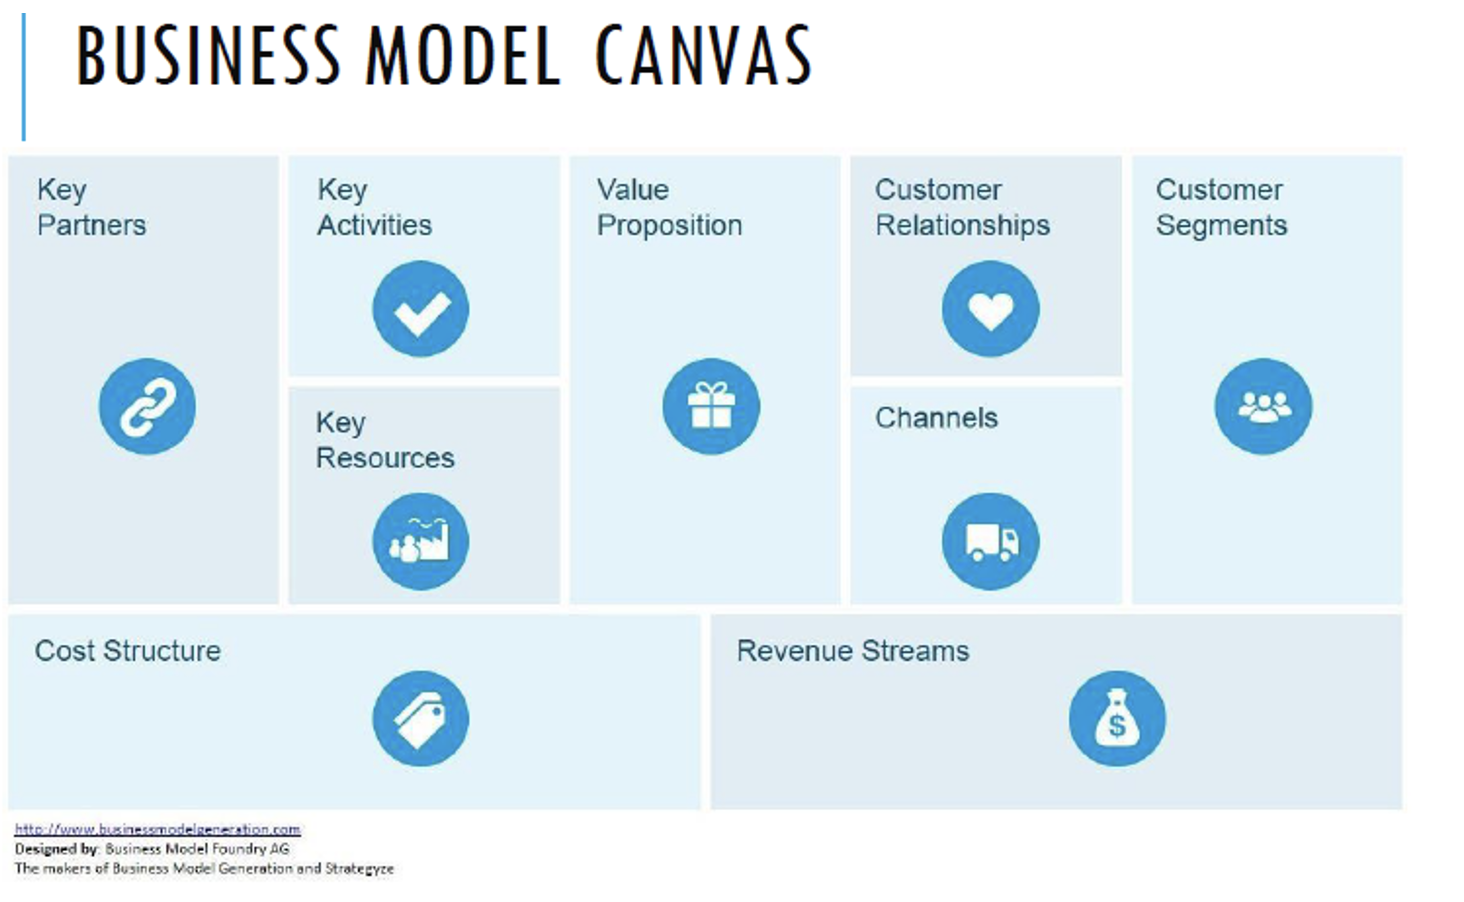
\includegraphics[width=0.8\textwidth]{imm/Screenshot 2026-09-10 alle 18.50.03.png}
    \caption{Business Model Canvas}
\end{figure}

These nine elements explain how a company creates, delivers, and captures value.

\section{1. Value Proposition}

The \textbf{value proposition} explains the value that a company offers to its customers and why customers should choose its product or service instead of competitors' alternatives.

The value proposition can be based on different factors, such as:
price, quality, convenience, innovation, performance, customization, design, brand, accessibility, and risk reduction.


A company can have \textbf{several value propositions} because different customer segments may have different needs and expectations.

The company should identify the value proposition that is the most profitable and sustainable for each target customer segment.

\subsection{Types of Value Propositions}
\begin{itemize}
    \item Novelty: The product or service is new and innovative, offering a unique solution to a problem or need.
    \item Performance: The product or service offers superior performance or functionality compared with competitors.
    \item Customization: The product or service can be tailored to meet the specific needs or preferences of individual customers.
    \item Design: The product or service has an appealing aesthetic or user experience that differentiates it from competitors.
    \item Brand / Status: The product or service is associated with a prestigious brand or represents a status symbol that increases its perceived value.
    \item Price: The product or service is offered at a competitive or affordable price that appeals to cost-conscious customers.   
    \item Convenience: The product or service is easy to access, use, or integrate into customers' lives, saving time or effort.
    \item Risk Reduction: The product or service reduces uncertainty or potential negative outcomes for customers,
    \item Accessibility: The product or service is made available to a wider range of customers, including customers with limited resources or special needs.
    \item Cost Reduction: The product or service helps customers save money or reduce expenses in the long term.
\end{itemize}


\section{2. Customer Segments (For Whom?)}

The \textbf{customer segment} is the group of people or organizations that a company aims to serve and for whom it creates value.

The market is divided into different groups of customers. These groups can have different needs, preferences, behaviors, and characteristics.

A segment can be identified according to:

\begin{itemize}
    \item \textbf{Demographics}: age, gender, income, education, occupation, etc.;
    \item \textbf{Psychographics}: lifestyle, personality, values, interests, etc.;
    \item \textbf{Behavior}: purchasing habits, frequency of use, brand loyalty, etc.;
    \item \textbf{Needs}: specific problems or requirements that customers want to solve.
\end{itemize}

A \textbf{market segment} is a group of people who respond in a similar way to a marketing strategy.

For example, engineering students and architecture students may represent different customer segments because they can have different needs and preferences.

The customer segment can also be divided into \textbf{sub-segments} based on specific characteristics or behaviors.

In a market, there are different customer groups, and the company chooses a \textbf{target segment} on which to focus.

The \textbf{target segment} is the group of customers that the company specifically aims to serve and create value for.

\subsection{Example: Ferrari}

\textbf{Ferrari} focuses strongly on quality, performance, luxury, exclusivity, and brand/status.

Its target customers are generally high-income individuals who value: high performance, luxury, exclusivity, prestige, and status.

The target segment can also be divided into smaller sub-segments according to customers' specific preferences and motivations.

For Ferrari, customers may be particularly interested in the \textbf{status and prestige} associated with owning the brand.

\section{3. Channels(  How Do We Get It to Them?)}

\textbf{Channels} describe how a company communicates with customers and how it delivers its value proposition to them.

Channels can be:
\begin{itemize}
    \item direct or indirect;
    \item online or offline;
    \item owned by the company or shared with other companies.
\end{itemize}

Examples of channels include: physical stores, websites, mobile applications, social media, email marketing, distributors, partners, marketplaces, events, traditional advertising, and print media.

The company has to choose the channel that is the most \textbf{effective and efficient} for each customer segment.

\subsection{Direct Channels}

A \textbf{direct channel} is a channel through which the company sells or communicates directly with customers.

Examples include:

\begin{itemize}
    \item a physical store owned by the company;
    \item the company's website;
    \item the company's mobile application;
    \item direct sales.
\end{itemize}

\subsection{Indirect Channels}

An \textbf{indirect channel} involves an intermediary between the company and the final customer.

Examples include: distributors, retailers, agents, business partners, and marketplaces.

\subsection{Owned and Partner Channels}

A company can use channels that it owns or channels shared with other companies.

For example:

\begin{itemize}
    \item an owned website is an \textbf{owned channel};
    \item a marketplace can be a \textbf{partner/shared channel}.
\end{itemize}

\subsection{Retail Store Example}

A \textbf{retail store} is a business that sells products directly to customers.

The retailer can buy products from another company and resell them to customers, generating revenue through a \textbf{markup} or commission.

For example:

\[
\text{Purchase Price} + \text{Markup} = \text{Selling Price}
\]

The retail store can be: physical, online, or both.

A retailer can also provide additional services such as: customer support, returns, exchanges, warranties, marketing and promotional activities, and loyalty programs.

The channels and customer relationships should be adapted to the specific needs and characteristics of the target segment.

\section{4. Customer Relationships}

\textbf{Customer relationships} describe the type of relationship that a company establishes and maintains with its customers.

Customer relationships can be:

\begin{itemize}
    \item personal or automated;
    \item transactional or long-term.
\end{itemize}

Examples include: personal assistance, dedicated personal assistance, self-service, automated services, loyalty programs, feedback systems, communities, and co-creation.

The company has to design the customer relationship that is most suitable for each customer segment.

For example, a cleaning-room worker and a university teacher may have very different needs and preferences. Therefore, the company may need to use different channels and customer relationships for different customer segments.

\section{5. Revenue Streams}

\textbf{Revenue streams} are the sources of income that a company generates from its business activities.

They explain \textbf{how the company makes money}.

Revenue streams can be based on different pricing models, such as:  one-time sales, recurring subscriptions, licensing fees, advertising revenue, usage fees, and commissions.


Different customer segments or different value propositions can generate different revenue streams.

For example:

\[
\text{Revenue} = \text{Price} \times \text{Quantity Sold}
\]

However, a company may also generate recurring revenues through subscriptions or usage-based pricing.

\section{6. Key Resources}

\textbf{Key resources} are the assets that a company needs to create, deliver, and capture value.

Key resources can be classified into four main categories:

\begin{itemize}
    \item \textbf{Physical resources};
    \item \textbf{Intellectual resources};
    \item \textbf{Human resources};
    \item \textbf{Financial resources}.
\end{itemize}


\subsection{Example: Electric Car Company}

To produce electric cars, a company needs different types of key resources.

\begin{itemize}
    \item \textbf{Physical}: factories, machinery, batteries, raw materials;
    \item \textbf{Intellectual}: patents, designs, software, technology;
    \item \textbf{Human}: engineers, designers, technicians;
    \item \textbf{Financial}: capital, loans, and investments.
\end{itemize}

Key resources can be owned by the company or accessed through partnerships and outsourcing.

\section{7. Key Activities}

\textbf{Key activities} are the most important actions that a company must perform to create and deliver its value proposition, reach customers, and generate revenues.

Examples of key activities include:

\begin{itemize}
    \item production;
    \item research and development;
    \item marketing;
    \item sales;
    \item distribution;
    \item problem solving;
    \item platform management;
    \item customer support.
\end{itemize}

The key activities depend on the company's business model.

For example, for a manufacturing company, production may be one of the most important activities. For a technology company, software development and research may be more important.

\section{8. Key Partnerships}

\textbf{Key partnerships} are strategic alliances that a company forms with other organizations in order to improve its capabilities, reduce risks, access resources, or reach new markets.

Key partners can include: suppliers, distributors, technology providers, research institutions, joint-venture partners, and other companies.


These partnerships can help the company ensure a reliable supply chain, efficient charging infrastructure, and advanced vehicle features.

A company can start without key partnerships, but partnerships can become important when the company needs external resources, expertise, technology, distribution, or risk sharing.

\subsection{Four Types of Partnerships}

There are four main types of partnerships:

\subsubsection{1. Strategic Alliances Between Non-Competitors}

Two companies that operate in different industries or markets collaborate to achieve mutual benefits.

They are not direct competitors but can complement each other's activities.

\subsubsection{2. Coopetition: Strategic Partnerships Between Competitors}

Two companies that operate in the same industry or market collaborate to achieve common goals.

Examples include:

\begin{itemize}
    \item joint research and development;
    \item shared marketing campaigns;
    \item co-branding;
    \item technology development.
\end{itemize}

This type of relationship can be described as \textbf{coopetition}, because companies cooperate while still competing in other areas.

\subsubsection{3. Joint Ventures}

Two or more companies create or participate in a separate business entity to pursue a specific project or business opportunity.

The partners share resources, risks, responsibilities, and potentially profits.

\subsubsection{4. Buyer-Supplier Relationships / Bottleneck Partnerships}

A company establishes a partnership with a supplier or another organization to secure access to an essential resource or overcome a specific constraint.


\section{9. Cost Structure}

The \textbf{cost structure} describes all the costs and expenses that a company incurs in order to operate its business model.

It includes the costs associated with: key resources, key activities, key partnerships, production, distribution, marketing, customer relationships, and administration.
The cost structure can be divided into different types.
\begin{figure}[H]
    \centering
    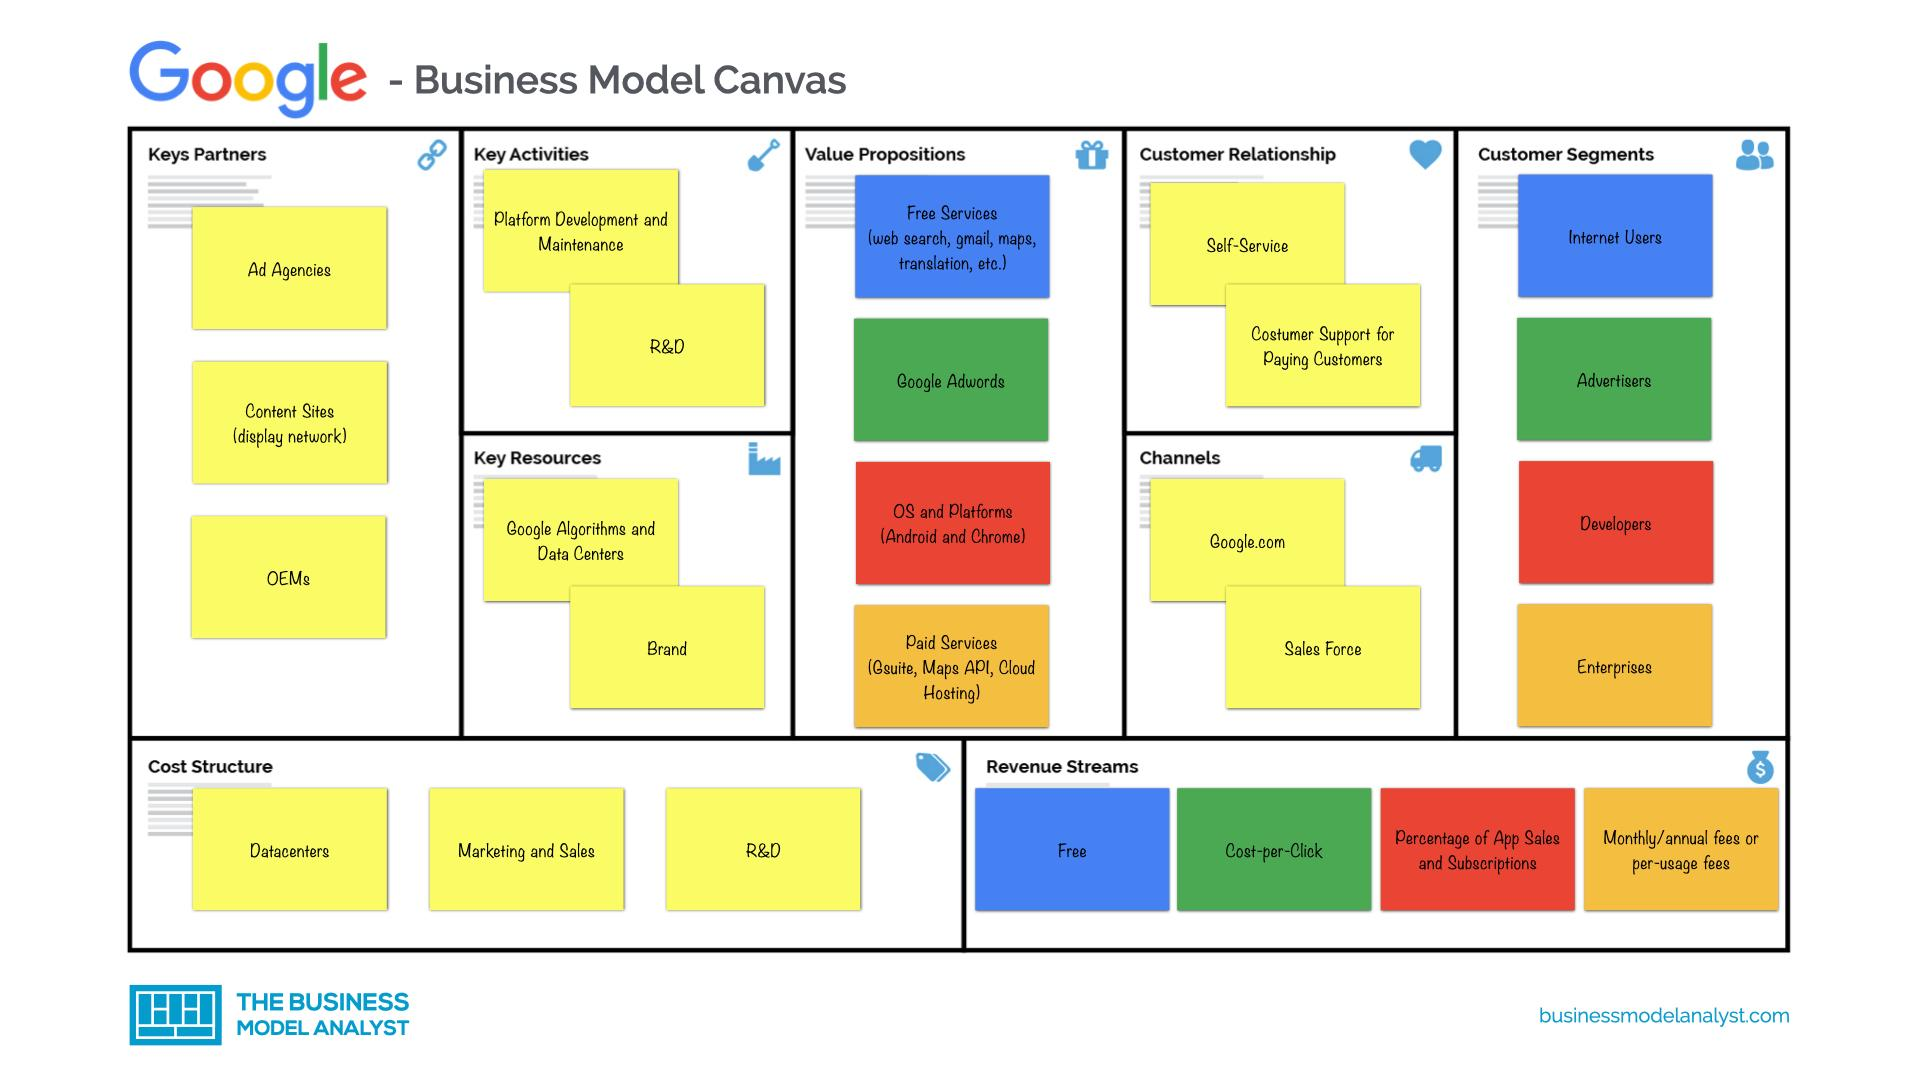
\includegraphics[width=1\textwidth]{imm/Google-Business-Model-Canvas.jpeg}
    \caption{Cost Structure}
\end{figure}
\end{document}